\documentclass[aspectratio=169]{beamer}
\usetheme{Madrid}
\usecolortheme{whale}
\definecolor{coforgenavy}{RGB}{13,40,79}
\definecolor{coforgeaccent}{RGB}{0,120,180}
\definecolor{c4person}{RGB}{8,56,113}
\definecolor{c4container}{RGB}{35,116,200}
\definecolor{c4external}{RGB}{140,140,140}
\setbeamercolor{structure}{fg=coforgenavy}
\setbeamercolor{title}{fg=white,bg=coforgenavy}
\setbeamercolor{frametitle}{fg=white,bg=coforgenavy}
\setbeamercolor{block title}{fg=white,bg=coforgeaccent}
\setbeamerfont{frametitle}{series=\bfseries}
\setbeamertemplate{navigation symbols}{}
\setbeamertemplate{footline}{%
  \hbox{\begin{beamercolorbox}[wd=1\paperwidth,ht=2.5ex,dp=1.2ex,leftskip=1em,rightskip=1em]{structure}
  \footnotesize Team Qudit Creons --- TechCon Hackathon \hfill Use Case \#47 \hfill \insertframenumber/\inserttotalframenumber
  \end{beamercolorbox}}%
}
\usepackage[utf8]{inputenc}
\usepackage{tikz}
\usetikzlibrary{arrows.meta, positioning, shapes.geometric, shadows}

\title[Mule Network Detection --- Stage 3]{Enterprise AI Platform for Scam, Mule Network \& \\ Suspicious Transaction Detection}
\subtitle{Use Case \#47 --- Stage 3 Evaluation, TechCon Hackathon, Coforge}
\author{Team Qudit Creons \\[0.3em] \small Abhishek Raj \quad \textbar\quad Divyansh Singh}
\institute{Coforge --- \#CoforgeTechCon2026 \quad \#CoforgeHackathon}
\date{Stage 3 Evaluation --- 1--2 September 2026}

\begin{document}

\begin{frame}
\titlepage
\end{frame}

% ---------------------------------------------------------
\begin{frame}{Vision \& The Problem}
\begin{block}{Vision Statement}
Give fraud investigators an explainable, real-time view of mule networks and scam patterns --- so suspicious money movement is stopped \emph{before cash-out}, not reconstructed after the loss.
\end{block}

\vspace{0.5em}
\textbf{Why network-first, not rule-per-transaction:} Fraud losses are driven by \emph{networks} of mule accounts moving funds in coordinated patterns --- fan-out smurfing, fan-in aggregation, layering chains, rapid pass-through. Row-level rules miss the shape; investigators can't trace it manually at scale.
\end{frame}

% ---------------------------------------------------------
\begin{frame}{Stakeholders}
\small
\begin{columns}[T]
\begin{column}{0.5\textwidth}
\textbf{Direct users}
\begin{itemize}
\item \textbf{Investigators} --- ranked queue, explainable evidence, network context
\item \textbf{Compliance officers} --- auditable reasoning, SAR-ready typology language
\item \textbf{Bank customers} --- fraud stopped fast; legitimate activity not disrupted
\end{itemize}
\end{column}
\begin{column}{0.5\textwidth}
\textbf{Governance \& infra}
\begin{itemize}
\item \textbf{Regulators} --- demonstrable due diligence, audit trail by construction
\item \textbf{Bank IT/Security} --- open-source stack, API-first, no core-banking rebuild
\item \textbf{Leadership} --- quantifiable precision gain = investigator-hours saved
\end{itemize}
\end{column}
\end{columns}
\end{frame}

% ---------------------------------------------------------
\begin{frame}{Architecture --- C4 Container Diagram}
\centering
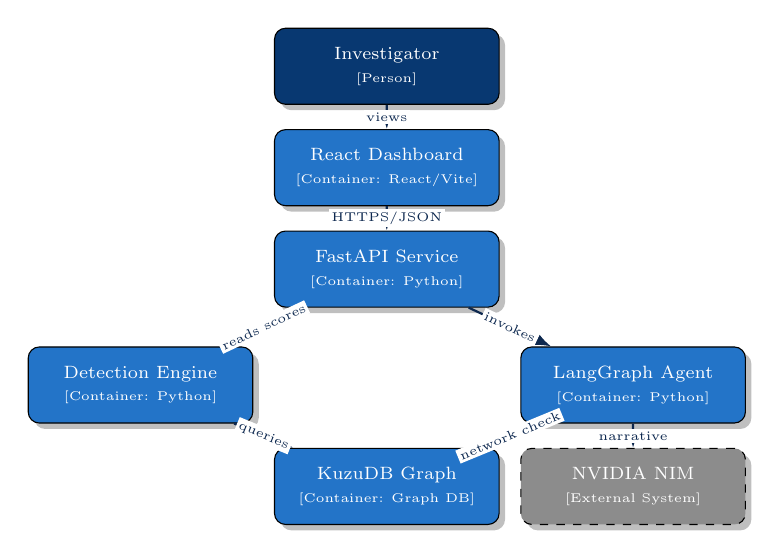
\begin{tikzpicture}[scale=0.92, every node/.style={scale=0.92},
  person/.style={draw, rounded corners, fill=c4person, text=white, minimum width=3.1cm, minimum height=1.05cm, align=center, font=\scriptsize, drop shadow},
  container/.style={draw, rounded corners, fill=c4container, text=white, minimum width=3.1cm, minimum height=1.05cm, align=center, font=\scriptsize, drop shadow},
  external/.style={draw, rounded corners, dashed, fill=c4external, text=white, minimum width=3.1cm, minimum height=1.05cm, align=center, font=\scriptsize, drop shadow},
  arr/.style={-{Latex[length=2mm]}, thick, coforgenavy},
  lbl/.style={font=\tiny, fill=white, inner sep=1pt}
]

\node[person]    (inv)    at (4.2, 6.0)  {Investigator\\[1pt]\tiny [Person]};
\node[container] (dash)   at (4.2, 4.6)  {React Dashboard\\[1pt]\tiny [Container: React/Vite]};
\node[container] (api)    at (4.2, 3.2)  {FastAPI Service\\[1pt]\tiny [Container: Python]};
\node[container] (detect) at (0.8, 1.6)  {Detection Engine\\[1pt]\tiny [Container: Python]};
\node[container] (agent)  at (7.6, 1.6)  {LangGraph Agent\\[1pt]\tiny [Container: Python]};
\node[container] (graph)  at (4.2, 0.2)  {KuzuDB Graph\\[1pt]\tiny [Container: Graph DB]};
\node[external]  (nim)    at (7.6, 0.2)  {NVIDIA NIM\\[1pt]\tiny [External System]};

\draw[arr] (inv) -- (dash) node[lbl, midway] {views};
\draw[arr] (dash) -- (api) node[lbl, midway] {HTTPS/JSON};
\draw[arr] (api) -- (detect) node[lbl, midway, sloped] {reads scores};
\draw[arr] (api) -- (agent) node[lbl, midway, sloped] {invokes};
\draw[arr] (detect) -- (graph) node[lbl, midway, sloped] {queries};
\draw[arr] (agent) -- (graph) node[lbl, midway, sloped] {network check};
\draw[arr] (agent) -- (nim) node[lbl, midway] {narrative};

\end{tikzpicture}

\vspace{-0.2em}
\footnotesize \textbf{C4 model, Container level.} Solid = internal container, dashed = external system, dark-blue = person actor. Full stack open-source except the NIM inference call.
\end{frame}

% ---------------------------------------------------------
\begin{frame}{Key Design Decisions}
\small
\begin{description}
\item[Rule-based, not GNN] Every flag explainable by construction --- no post-hoc SHAP/GNNExplainer needed to justify a regulatory decision; no training data required.
\item[KuzuDB, not Neo4j] Embedded, no JVM overhead --- matters on constrained dev/cloud hardware; team had zero prior Cypher experience either way.
\item[Relative thresholds, not fixed] Self-calibrated per account. \emph{Proven necessary}: our fixed-threshold detector hit 100\% false positives against Santander's independent \texttt{gen-fraud-graph} benchmark --- exposed real overfitting to our own dataset's shape.
\item[Damped corroboration scoring] Strongest single signal counts fully; weak coincidental signals don't stack to a false flag. Validated by injecting legitimate payroll/marketplace accounts and testing directly against them.
\end{description}
\end{frame}

% ---------------------------------------------------------
\begin{frame}{Validation Methodology --- Not Just a Demo}
\begin{itemize}
\item \textbf{Adversarial self-testing:} injected legitimate high-volume businesses (payroll processor, marketplace) into our own dataset and measured false positives on them directly --- found and fixed a real toy-model gap
\item \textbf{External benchmark validation:} ran our detectors, unmodified, against Santander AI Lab's independent open-source synthetic fraud graph --- surfaced a genuine generalization failure before it could surface in production
\item \textbf{Iterative, measured improvement:} every scoring change verified against the full evaluation suite before being kept; one regression caught and reverted the same session it was introduced
\end{itemize}

\vspace{0.5em}
\begin{block}{Result}
\centering
Precision: 0.746 $\rightarrow$ 0.855 \quad|\quad Recall: 1.000 (held throughout) \quad|\quad False Positives: 222 $\rightarrow$ 110
\end{block}
\end{frame}

% ---------------------------------------------------------
\begin{frame}{Live Demonstration}
\centering
\Large \textbf{Live system} --- \texttt{http://80.225.235.192:4173}

\vspace{1em}
\normalsize
\begin{itemize}
\item Deployed on Oracle Cloud (Ampere A1.Flex, 4 OCPU / 24GB, Always Free tier)
\item Running as managed systemd services --- survives reboots, not a laptop demo
\item Full pipeline live: flagged accounts $\rightarrow$ live KuzuDB drill-down $\rightarrow$ Nemotron case narrative $\rightarrow$ network-aware escalation
\end{itemize}
\end{frame}

% ---------------------------------------------------------
\begin{frame}{Business Value \& Roadmap}
\small
\begin{columns}[T]
\begin{column}{0.5\textwidth}
\textbf{Business value}
\begin{itemize}
\item Fewer false positives = fewer wasted investigator-hours
\item Zero missed fraud (recall 1.000) throughout every iteration
\item Explainable-by-design = lower regulatory/audit risk than black-box ML
\item Fully open-source stack = no vendor lock-in
\end{itemize}
\end{column}
\begin{column}{0.5\textwidth}
\textbf{Next steps}
\begin{itemize}
\item Continuous scoring for remaining two detectors (fan-out, layering)
\item True incremental/live ingestion (currently batch-refresh)
\item Formal held-out validation split (current eval is same-dataset)
\item Broader external benchmark coverage
\end{itemize}
\end{column}
\end{columns}
\end{frame}

% ---------------------------------------------------------
\begin{frame}
\centering
\Huge Thank You

\vspace{1em}
\Large Q\&A

\vspace{2em}
\normalsize Team Qudit Creons --- Abhishek Raj, Divyansh Singh \\
\texttt{github.com/Qyngshuk08/145-qudit-creons}
\end{frame}

\end{document}